\documentclass[notes,11pt, aspectratio=169]{beamer}

\usepackage{pgfpages}
% These slides also contain speaker notes. You can print just the slides,
% just the notes, or both, depending on the setting below. Comment out the want
% you want.
\setbeameroption{hide notes} % Only slide
%\setbeameroption{show only notes} % Only notes
%\setbeameroption{show notes on second screen=right} % Both

\usepackage{helvet}
\usepackage[default]{lato}
\usepackage{array}
\usepackage{tgbonum}

\usepackage{tikz}
\usepackage{verbatim}
\setbeamertemplate{note page}{\pagecolor{yellow!5}\insertnote}
\usetikzlibrary{positioning}
\usetikzlibrary{snakes}
\usetikzlibrary{calc}
\usetikzlibrary{arrows}
\usetikzlibrary{decorations.markings}
\usetikzlibrary{shapes.misc}
\usetikzlibrary{matrix,shapes,arrows,fit,tikzmark}
\usepackage{amsmath}
\usepackage{mathpazo}
\usepackage{hyperref}
\usepackage{lipsum}
\usepackage{multimedia}
\usepackage{graphicx}
\usepackage{multirow}
\usepackage{graphicx}
\usepackage{dcolumn}
\usepackage{bbm}
\newcolumntype{d}[0]{D{.}{.}{5}}

\usepackage{changepage}
\usepackage{appendixnumberbeamer}
\newcommand{\beginbackup}{
   \newcounter{framenumbervorappendix}
   \setcounter{framenumbervorappendix}{\value{framenumber}}
   \setbeamertemplate{footline}
   {
     \leavevmode%
     \hline
     box{%
       \begin{beamercolorbox}[wd=\paperwidth,ht=2.25ex,dp=1ex,right]{footlinecolor}%
%         \insertframenumber  \hspace*{2ex} 
       \end{beamercolorbox}}%
     \vskip0pt%
   }
 }
\newcommand{\backupend}{
   \addtocounter{framenumbervorappendix}{-\value{framenumber}}
   \addtocounter{framenumber}{\value{framenumbervorappendix}} 
}


\usepackage{graphicx}
\usepackage[space]{grffile}
\usepackage{booktabs}
\newcommand\independent{\protect\mathpalette{\protect\independenT}{\perp}}
\def\independenT#1#2{\mathrel{\rlap{$#1#2$}\mkern2mu{#1#2}}}
\DeclareMathOperator{\Supp}{Supp}


\newtheorem{assN}{Assumption}
% These are my colors -- there are many like them, but these ones are mine.
\definecolor{blue}{RGB}{0,114,178}
\definecolor{red}{RGB}{213,94,0}
\definecolor{yellow}{RGB}{240,228,66}
\definecolor{green}{RGB}{0,158,115}

\hypersetup{
  colorlinks=false,
  linkbordercolor = {white},
  linkcolor = {blue}
}


%% I use a beige off white for my background
\definecolor{MyBackground}{RGB}{255,253,218}

%% Uncomment this if you want to change the background color to something else
%\setbeamercolor{background canvas}{bg=MyBackground}

%% Change the bg color to adjust your transition slide background color!
\newenvironment{transitionframe}{
  \setbeamercolor{background canvas}{bg=yellow}
  \begin{frame}}{
    \end{frame}
}

\setbeamercolor{frametitle}{fg=blue}
\setbeamercolor{title}{fg=black}
\setbeamertemplate{footline}[frame number]
\setbeamertemplate{navigation symbols}{} 
\setbeamertemplate{itemize items}{-}
\setbeamercolor{itemize item}{fg=blue}
\setbeamercolor{itemize subitem}{fg=blue}
\setbeamercolor{enumerate item}{fg=blue}
\setbeamercolor{enumerate subitem}{fg=blue}
\setbeamercolor{button}{bg=MyBackground,fg=blue,}



% If you like road maps, rather than having clutter at the top, have a roadmap show up at the end of each section 
% (and after your introduction)
% Uncomment this is if you want the roadmap!
% \AtBeginSection[]
% {
%    \begin{frame}
%        \frametitle{Roadmap of Talk}
%        \tableofcontents[currentsection]
%    \end{frame}
% }
\setbeamercolor{section in toc}{fg=blue}
\setbeamercolor{subsection in toc}{fg=red}
\setbeamersize{text margin left=1em,text margin right=1em} 

\newenvironment{wideitemize}{\itemize\addtolength{\itemsep}{10pt}}{\enditemize}

\usepackage{environ}
\NewEnviron{videoframe}[1]{
  \begin{frame}
    \vspace{-8pt}
    \begin{columns}[onlytextwidth, T] % align columns
      \begin{column}{.70\textwidth}
        \begin{minipage}[t][\textheight][t]
          {\dimexpr\textwidth}
          \vspace{8pt}
          \hspace{4pt} {\Large \sc \textcolor{blue}{#1}}
          \vspace{8pt}
          
          \BODY
        \end{minipage}
      \end{column}%
      \hfill%
      \begin{column}{.38\textwidth}
        \colorbox{green!20}{\begin{minipage}[t][1.2\textheight][t]
            {\dimexpr\textwidth}
            Face goes here
          \end{minipage}}
      \end{column}%
    \end{columns}
  \end{frame}
}

\title[]{\textcolor{blue}{Partial Identification}} \author[PGP]{}
\institute[FRBNY]{\small{\begin{tabular}{c}
                           Paul Goldsmith-Pinkham  \\
\end{tabular}}}

\date{\today}

\begin{document}

%%% TIKZ STUFF
\tikzset{   
        every picture/.style={remember picture,baseline},
        every node/.style={anchor=base,align=center,outer sep=1.5pt},
        every path/.style={thick},
        }
\newcommand\marktopleft[1]{%
    \tikz[overlay,remember picture] 
        \node (marker-#1-a) at (-.3em,.3em) {};%
}
\newcommand\markbottomright[2]{%
    \tikz[overlay,remember picture] 
        \node (marker-#1-b) at (0em,0em) {};%
}
\tikzstyle{every picture}+=[remember picture] 
\tikzstyle{mybox} =[draw=black, very thick, rectangle, inner sep=10pt, inner ysep=20pt]
\tikzstyle{fancytitle} =[draw=black,fill=red, text=white]
%%%% END TIKZ STUFF

% Title Slide
\begin{frame}
\maketitle
\end{frame}

\begin{frame}{Seeking Identification}
  \begin{wideitemize}
  \item For our questions, we need to describe an \emph{estimand} of
    interest
    \begin{itemize}
    \item This may be a causal object, or purely a statistical one
    \end{itemize}
    \item Remember that we need to know whether this object is knowable
      given the data generating process
      \begin{itemize}
      \item This is not a question of any given sample, but rather a
        question of our underlying assumptions and the data generating
        process
      \end{itemize}
    \item Two examples:
      \begin{itemize}
      \item When were only observe a subsample of outcomes for
        individuals, we assume the data is missing (completely) at
        random to identify the full population's average
      \item To identify the average treatment effect, we
        assumed strict ignorability (and a few other things) to
        identify the effect of the treatment
      \end{itemize}
    \item Can we assume less?
  \end{wideitemize}
\end{frame}

\begin{frame}{Start with a simple example}
  \begin{wideitemize}
  \item The housing market is extremely hot and you want to know what
    the probability that a house sells $(Y_{i} = 1)$ vs doesn't sell $(Y_{i} = 0)$
    \begin{itemize}
  \item In particular, you want to know if houses with backyards
    $(X_{i} = 1)$ are selling more quickly than those without
    $(X_{i} = 0)$.
  \end{itemize}
\item However, we only observe a sale for the set of homes that chose
  to go on the market $Z_{i} = 1$ and do not observe $Y_{i}$ for
  $Z_{i} = 0$
  \begin{itemize}
  \item Can we know the probability of sale $E(Y_{i} | X_{i})$ for all houses? 
  \end{itemize}
\item Formally, assume that we will have a dataset of $n$ independent
  triplets $(Y_{i}, X_{i}, Z_{i})$
  \begin{itemize}
  \item $E(Y_{i} | X_{i}, Z_{i} = 1)$ is identified but
    $E(Y_{i} | X_{i})$ is not without more assumptions
  \end{itemize}
\item But $E(Y_{i} | X_{i})$ is \emph{partially} identified
  \end{wideitemize}
\end{frame}

\begin{frame}{Simple parital identification example}
  \begin{wideitemize}
  \item Consider the law of total probability:
    \begin{align*}
      E(Y_{i} | X_{i} ) = Pr(Y_{i} = 1 |X_{i}) &= Pr(Y_{i} = 1 | X_{i}, Z_{i} = 1)  \times Pr(Z_{i} = 1 | X_{i}) \\
      & + Pr(Y_{i} = 1 | X_{i}, Z_{i} = 0)  \times Pr(Z_{i} = 0 | X_{i}) 
    \end{align*}
  \item The problem is we cannot observe $Pr(Y_{i} = 1 | X_{i}, Z_{i} = 0)$, by definition
    \begin{itemize}
    \item But, we know that it cannot be greater than one, nor less than zero
    \end{itemize}
  \item As a result, it must be that
    \begin{align*}
      E(Y_{i} | X_{i} ) \in &  [Pr(Y_{i} = 1 | X_{i}, Z_{i} = 1)  \times Pr(Z_{i} = 1 | X_{i}), \\
      & Pr(Y_{i} = 1 | X_{i}, Z_{i} = 1)  \times Pr(Z_{i} = 1 | X_{i}) + Pr(Z_{i} = 0 | X_{i})]
    \end{align*}
  \item This is intuitive! For all the houses we don't see go for
    sale, at the extreme, they could either all \emph{not} sell (the
    lower bound) or all sell (the upper bound). 
  \end{wideitemize}
\end{frame}

\begin{frame}{Simple partial identification example}
  \begin{wideitemize}
  \item This is quite powerful -- we've made no assumptions on the
    correlation between the choice to sell and sale probability.
    \begin{itemize}
    \item The width of this interval is important -- it speaks to the
      informativeness of the bound (and in this case is equal to
      $Pr(Z_{i} = 0 | X_{i})$
    \item The more likely properties are to sell, the tighter these
      bounds become (since the missing piece gets smaller)
    \end{itemize}
  \item What does a missing-at-random assumption imply?
    \begin{itemize}
    \item $Pr(Y_{i} = 1 | X_{i}, Z_{i} ) = Pr(Y_{i} = 1 | X_{i})$,
      which means that you can ignore the missing data and the set
      interval becomes a single point
    \item Hence, point identification!
    \end{itemize}
  \end{wideitemize}
\end{frame}

\begin{frame}{Simple partial identification example}
  \begin{wideitemize}
  \item A few things worth noting from this simple example
  \item First, what if $Y_{i}$ wasn't binary, but was real valued?
    E.g. sale price?
    \begin{itemize}
    \item If the value of $Y_{i}$ is unbounded, the upper bound of the
      set would be infinity
    \end{itemize}
    \item However, even with unbounded $Y_{i}$, you can always bound
      the CDF of $Y_{i}$ at different points: $F(Y_{i} \leq t)$ is
      always between 0 and 1
      \begin{itemize}
      \item This means we can set identify quantiles of the distribution!
      \item Recall that this came up when discussing censored data
      \end{itemize}
    \item So long as there is sufficient observed data, Manski (1994)
      shows that the $\alpha$ quantile is bounded by:
      \begin{itemize}
      \item Below:  $[\alpha - P(Z_{i} = 0 | X)] / P(Z_{i} = 1 | X)$-quantile of
        the observed distribution $Pr(Y_{i} | X_{i}, Z_{i} = 1)$ (if $Pr(Z_{i} = 0 | X_{i}) \leq \alpha$, and the min of $Y_{i}$ otherwise)
      \item Above:  $\alpha / P(Z_{i} = 1 | X)$-quantile of
        the observed distribution $Pr(Y_{i} | X_{i}, Z_{i} = 1)$ (if $Pr(Z_{i} = 0 | X_{i}) \leq 1- \alpha$, and the max of $Y_{i}$ otherwise)
      \end{itemize}
  \end{wideitemize}
\end{frame}

\begin{frame}{Back to generality: partial identification}
  \begin{wideitemize}
  \item Bounds are extremely powerful -- we can make substantially
    fewer assumptions and still potentially learn quite a bit
  \item However, it's worth noting that these are quite limited in practice
    \begin{itemize}
    \item Today, I will walk through two examples where I think they are quite valuable
    \end{itemize}
  \item Then we'll discuss why these might have had limited adoption
  \item We will ignore inference, although it is quite important (and
    has a big econometrics field associated with it)
    \begin{itemize}
    \item See Imbens and Manski (2004) and Chernozhukov, Hong and Tamer (2007) for initial primers
    \end{itemize}
  \end{wideitemize}
\end{frame}

\begin{frame}{Selection into employment}
      \begin{columns}[onlytextwidth, T] % align columns
        \begin{column}{.9\textwidth}
          \begin{wideitemize}
          \item Consider the problem of estimating the effect of a
            treatment (job training) on \emph{wages}
          \item Remember that the decision to work is a sample
            selection problem, even when you have an RCT!
          \item E.g., we only observe the wages of those who choose to
            work -- there may be endogeneous decisions to not work due
            to the treatment
          \item As a result, we have both the potential wage outcomes
            due to $D$: $(Y^{*}(0), Y^{*}(1))$ but \emph{also} the
            decision to work $S(0), S(1)$. Note that we don't observe
            $Y^{*} = D_{i}Y^{*}(1) + (1-D_{i})Y^{*}(0)$ if $S = 0$.
          \item This is a serious issue that plagues almost all
            research designs
            \begin{itemize}
            \item Many papers get around this by looking at ``total
              earnings'' to avoid wages
            \end{itemize}
          \end{wideitemize}
      \end{column}%
      \hfill%
      \begin{column}{.5\textwidth}
      \end{column}%
    \end{columns}
\end{frame}


\begin{frame}{Lee Bounds (Lee 2009)}
      \begin{columns}[onlytextwidth, T] % align columns
        \begin{column}{.5\textwidth}
          \begin{wideitemize}
          \item Lee 2009 considers this problem, and proposes
            sharp bounds
          \item The problem boils down to the following issue: when
            you treat someone, do you change their employment status?
            \begin{itemize}
            \item If no, the $S_{i}(1) = S_{i}(0)$ and there is no
              selection problem
            \item If yes, the $S_{i}(1) \not= S_{i}(0)$ and the
              question is where do the marginal ``shifters'' come from
              and end up in the outcome distribution?
            \end{itemize}
            \vspace{-6pt}
          \item E.g. if those who are induced to not work because they
            go to school b/c they get high returns from schooling,
            then this is negatively selecting away from the top part
            of the $Y^{*}(1)$ distribution
          \end{wideitemize}
      \end{column}%
      \hfill%
      \begin{column}{.5\textwidth}
        
\includegraphics[width=\linewidth]{images/lee_1.png}
      \end{column}%
    \end{columns}
\end{frame}


\begin{frame}{Lee Bounds (Lee 2009)}
      \begin{columns}[onlytextwidth, T] % align columns
        \begin{column}{.9\textwidth}
          \begin{wideitemize}
          \item Hopefully the problem sounds familiar (IV + LATE)
            \begin{itemize}
            \item The solution is similar too
            \end{itemize}
          \item Under monotonicity of selection (
            $S_{i}(1) \geq S_{i}(0)$, it is possible to provide sharper
            bounds on the treatment effect
          \item Let $\tau = E(Y^{*}(1) - Y^{*}(0) | S(0) = 1, S(1) = 1)$, our estimand of interest, and $p_{0} = \frac{Pr(S = 1 | D = 1) - Pr(S = 1| D = 0)}{Pr(S = 1 | D = 1)}$ 
          \item Then, we can bound $\tau \in [\Delta_{0}^{LB}, \Delta_{0}^{UB}]$
            \begin{itemize}
            \item $\Delta_{0}^{LB} = E(Y | D = 1, S = 1, Y \leq y_{1-p_{0}}) - E(Y | D = 0, S = 1)$
            \item $\Delta_{0}^{UB} = E(Y | D = 1, S = 1, Y \geq y_{p_{0}}) - E(Y | D = 0, S = 1)$
            \item where $y_{p_{0}}$ is the $p_{0}$th quantile
            \end{itemize}
          \end{wideitemize}
      \end{column}%
      \hfill%
      \begin{column}{.5\textwidth}

      \end{column}%
    \end{columns}
\end{frame}

\begin{frame}{Lee Bounds}
  \begin{wideitemize}
  \item We can bound $\tau \in [\Delta_{0}^{LB}, \Delta_{0}^{UB}]$
    \begin{itemize}
    \item $\Delta_{0}^{LB} = E(Y | D = 1, S = 1, Y \leq y_{1-p_{0}}) - E(Y | D = 0, S = 1)$
    \item $\Delta_{0}^{UB} = E(Y | D = 1, S = 1, Y \geq y_{p_{0}}) - E(Y | D = 0, S = 1)$
    \item where $y_{p_{0}}$ is the $p_{0}$th quantile
    \end{itemize}
  \item This has a number of cool properties:
    \begin{enumerate}
    \item If $p_{0} \to 0$, under monotonicity that means no sample
      selection. It also provides a test of mononicity: if covariates
      shift between treated and control with $p_{0} = 0$ and $S = 1$,
      then monotonicity likely fails if the selection is predictable based on covariates
    \item This is very similar to the always-take and complier analogy
      \begin{itemize}
      \item The bounds are exploiting the ``worst case'' scenarios --
        if the group of ``shifters'' are the ``best'' $Y(1)$, then
        trimming the top provides a lower bound.
      \item If the ``shifters'' are the worst, then trimming the bottom
        provides the upper bound
      \end{itemize}
    \item Using covariates can be used to narrow these bounds by shrinking the size of $p_{0}$
    \end{enumerate}
  \end{wideitemize}
\end{frame}

\begin{frame}{Lee Bounds (Lee 2009)}
      \begin{columns}[onlytextwidth, T] % align columns
        \begin{column}{.8\textwidth}
          \begin{wideitemize}
          \item Why is this approach great?
            \begin{itemize}
            \item No additional instrument or model needed
            \item Just monotonicity
            \item Can also work in broader sample selection questions
              -- not just wage selection, but sample attrition and
              other problems (recall the RD bunching approach!)
            \end{itemize}
          \item This approach is tighter than the general
            Horowitz-Manski bounds (analogous to what we discussed at
            start of today's class)
            \begin{itemize}
            \item Why? Monoticity restriction gets you a lot of power
            \item Without that assumption, bounds are extremely wide
              (because the outcome is unbounded)
            \end{itemize}
          \item Implemented in Stata (\texttt{leebounds}) and R
            (\texttt{leebounds})
          \end{wideitemize}
      \end{column}%
      \hfill%
      \begin{column}{.5\textwidth}
      \end{column}%
    \end{columns}
\end{frame}

\begin{frame}{Follow-up: Better Lee Bounds (Semenova 2020)}
      \begin{columns}[onlytextwidth, T] % align columns
        \begin{column}{.5\textwidth}
          \begin{wideitemize}
          \item Makes covariate usage easier and relaxes monotonicity condition to be conditional on
            covariates (potentially high dimensional)
            \begin{itemize}
            \item Lee bounds require a positive number of treated and
              control outcomes for each covariate value
            \item Challenging with continuous values, or many
            \end{itemize}
          \item Asymptotically sharp under ``many'' covariates 
          \item Code: \url{https://github.com/vsemenova/leebounds}
          \end{wideitemize}
      \end{column}%
      \hfill%
      \begin{column}{.5\textwidth}
        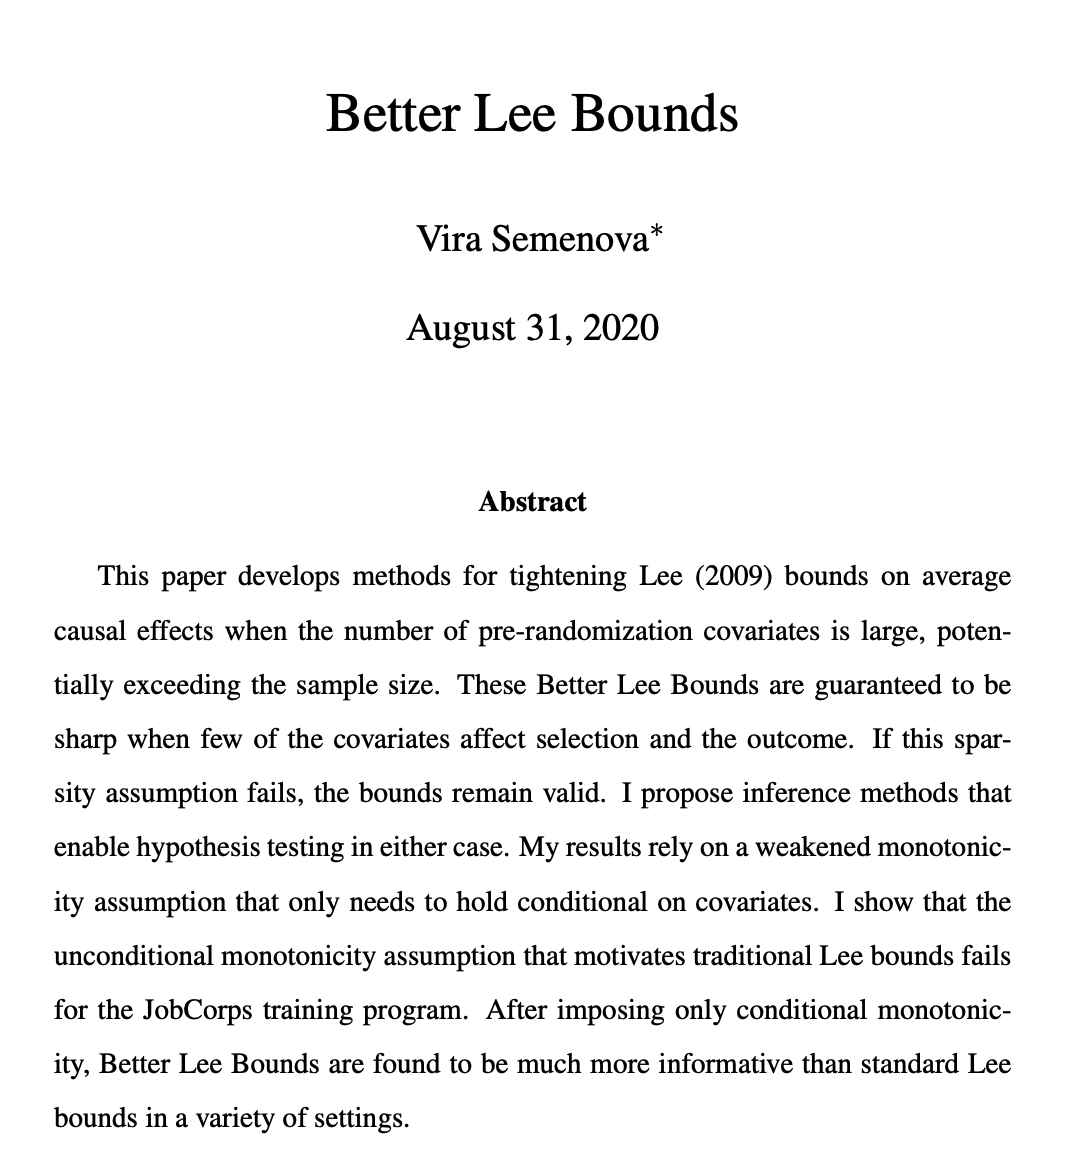
\includegraphics[width=\linewidth]{images/semenova_1.png}
      \end{column}%
    \end{columns}
\end{frame}


\begin{frame}{Manski and Tamer (2002)}
      \begin{columns}[onlytextwidth, T] % align columns
        \begin{column}{.5\textwidth}
          \begin{wideitemize}
          \item In many survey settings, data is not reported exactly, but instead in bounds
            \begin{itemize}
            \item Wealth may be reported in ranges to encourage participation
            \item Or, data may be supressed into bins to preserve
              anonymity (e.g. County Business Patterns data on
              employment)
            \end{itemize}
          \item By definition, theis interval data should lead to
            set-identified parameters
            \begin{itemize}
            \item Manski and Tamer (2002) is exactly concerned with this question
            \end{itemize}
          \end{wideitemize}
      \end{column}%
      \hfill%
      \begin{column}{.5\textwidth}
        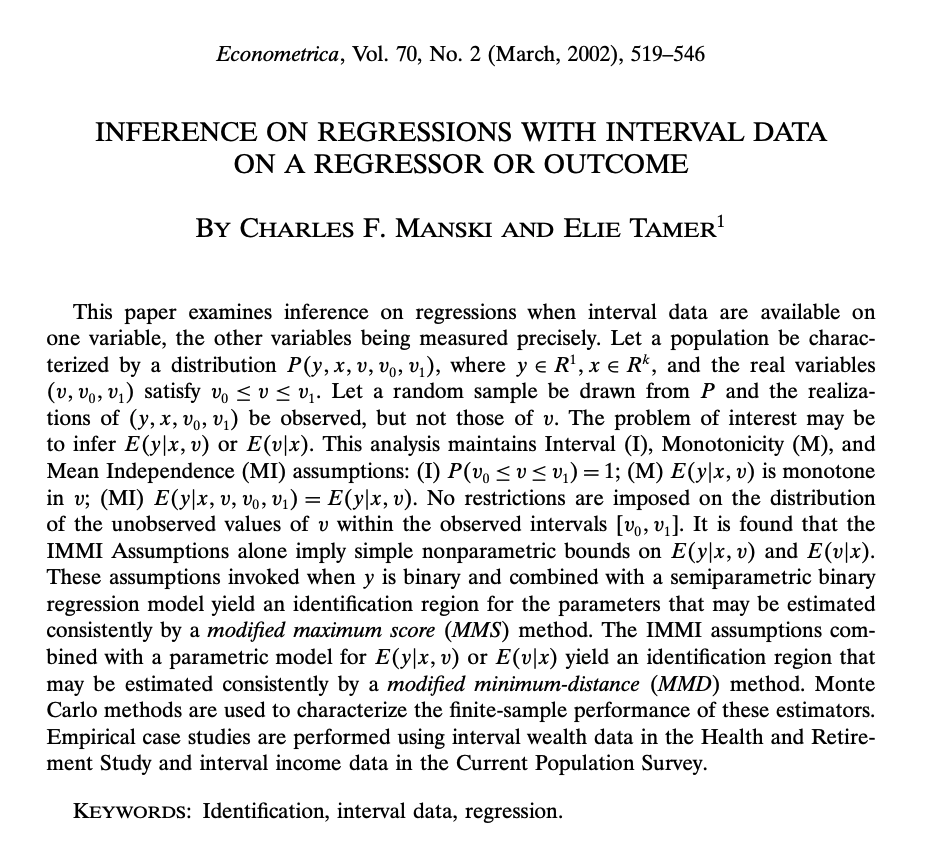
\includegraphics[width=\linewidth]{images/manski_tamer_1.png}
      \end{column}%
    \end{columns}
\end{frame}


\begin{frame}{Manski and Tamer (2002)}
      \begin{columns}[onlytextwidth, T] % align columns
        \begin{column}{.9\textwidth}
          \begin{wideitemize}
          \item Consider the data $(y, v, v_{0}, v_{1},x)$, where $v$ is
            the true measure you'd like, which is reported with
            intervals $[v_{0},v_{1}]$. 
          \item Manski and Tamer (2002) assume:
            \begin{enumerate}
            \item $E(Y|v,x) $ is weakly monotonic in $v$
            \item $E(Y|v, x,v_{0},v_{1})= E(Y|v,x)$
            \end{enumerate}
          \item In these settings, it is possible to put sharp bounds
            on the coefficients of a linear model
            \begin{itemize}
            \item Important to note -- in a multivariate regression,
              the set interval data on the right-hand side will also
              affect the coefficients for non-set interval data
            \end{itemize}
          \item Can also be adopted to study $E(v | x)$ for covariates $x$
            \begin{itemize}
            \item There are \emph{many} data sources with type of set interval nature!
            \end{itemize}
          \end{wideitemize}
      \end{column}%
      \hfill%
      \begin{column}{.5\textwidth}
      \end{column}%
    \end{columns}
\end{frame}


\begin{frame}{Excellent application considering interval data: Novosad, Rafkin and Asher (2022)}
      \begin{columns}[onlytextwidth, T] % align columns
        \begin{column}{.5\textwidth}
          \begin{wideitemize}
          \item Mortality rates among non-Hispanic Whites without college degrees have
            increased substantially over time
            \begin{itemize}
            \item Why?
            \end{itemize}
          \item Three possible reasons:
            \begin{itemize}
            \item an artifact of shifts in the education
              distribution
            \item mortality could be rising uniformly among
              individuals in the bottom half of the education dist
            \item mortality could be rising substantially at the very
              bottom of the education distribution
            \end{itemize}
          \end{wideitemize}
      \end{column}%
      \hfill%
      \begin{column}{.5\textwidth}
        \only<1>{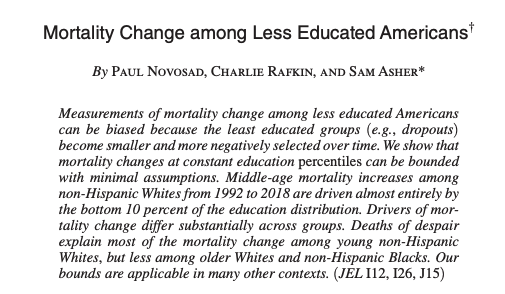
\includegraphics[width=\linewidth]{images/novosad1.png}       }
        \only<2>{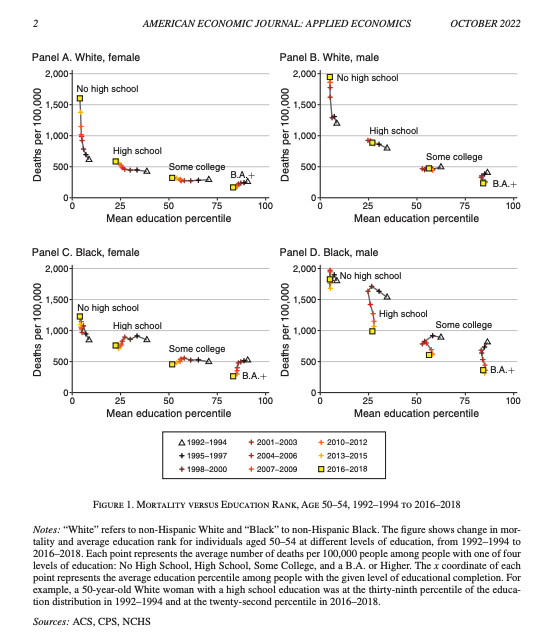
\includegraphics[width=\linewidth]{images/novosad2.png}       }        
      \end{column}%
    \end{columns}
\end{frame}


\begin{frame}{Excellent application considering interval data: Novosad, Rafkin and Asher (2022)}
      \begin{columns}[onlytextwidth, T] % align columns
        \begin{column}{.5\textwidth}
          \begin{wideitemize}
          \item This paper uses Manski and Tamer with two additional assumptions:
            \begin{enumerate}
            \item there exists a latent
              education rank, which is only coarsely observed in the
              education data
            \item mortality rate is weakly decreasing in the latent
              education rank
            \end{enumerate}
          \item Effectively, put bounds on $E(y | x \in [a,b])$
          \end{wideitemize}
      \end{column}%
      \hfill%
      \begin{column}{.5\textwidth}
        \only<1>{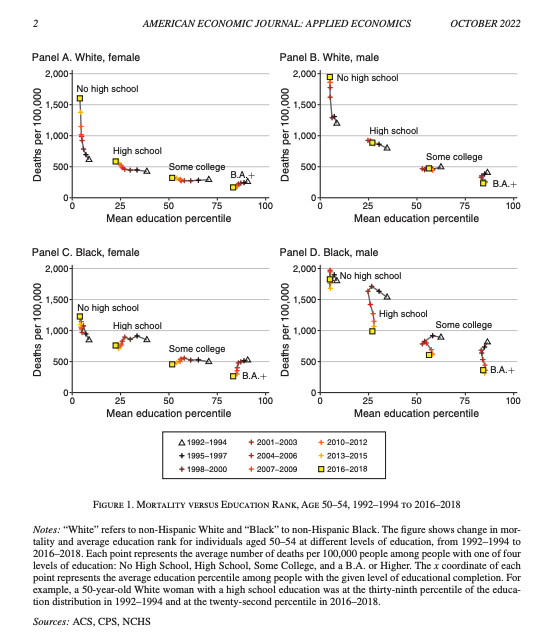
\includegraphics[width=\linewidth]{images/novosad2.png}       }
        \only<2>{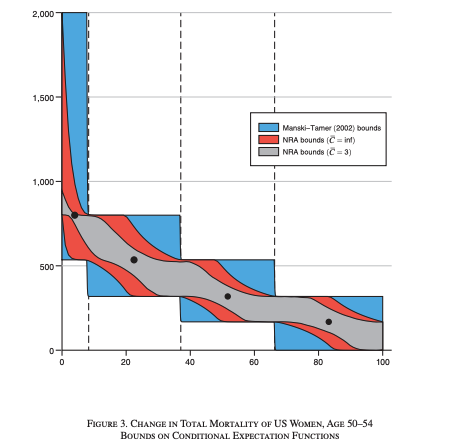
\includegraphics[width=\linewidth]{images/novosad3.png}       }
        \only<3>{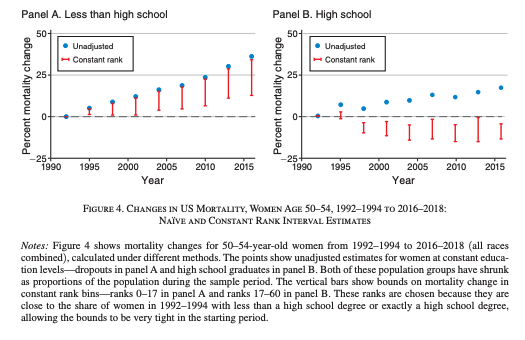
\includegraphics[width=\linewidth]{images/novosad4.png}       }
        \only<4>{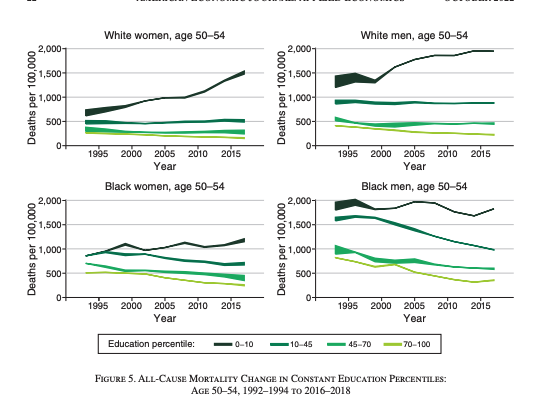
\includegraphics[width=\linewidth]{images/novosad5.png}       }                        
      \end{column}%
    \end{columns}
\end{frame}




\begin{frame}{Other things?}
  \begin{wideitemize}
  \item Both of these approaches are very practical ways to deal with
    data issues
  \item They also give a hint about how to think about these
    applications in other settings
    \begin{itemize}
    \item We are only scratching the surface of partial ID settings today!
    \end{itemize}
  \item Are there other useful applications worth considering?
    \begin{itemize}
    \item A major set related to modeling: many structural economic
      models imply inequalities for parameters of interest, which lead
      to set identification
    \item What about using shape assumptions on treatments?
    \end{itemize}
  \end{wideitemize}

\end{frame}

% \begin{frame}{Monotone Treatment Response  (Manski 1997)}
%       \begin{columns}[onlytextwidth, T] % align columns
%         \begin{column}{.5\textwidth}
%           \begin{wideitemize}
%           \item Consider treatment $D \in \{0,1\}$ -- assume that
%             $Y_{i}(1) \geq Y_{i}(0)$
%             \begin{itemize}
%             \item \emph{shape} restriction on the function $Y$
%             \end{itemize}
%           \item What can we learn?
            
%           \end{wideitemize}
%       \end{column}%
%       \hfill%
%       \begin{column}{.5\textwidth}
%         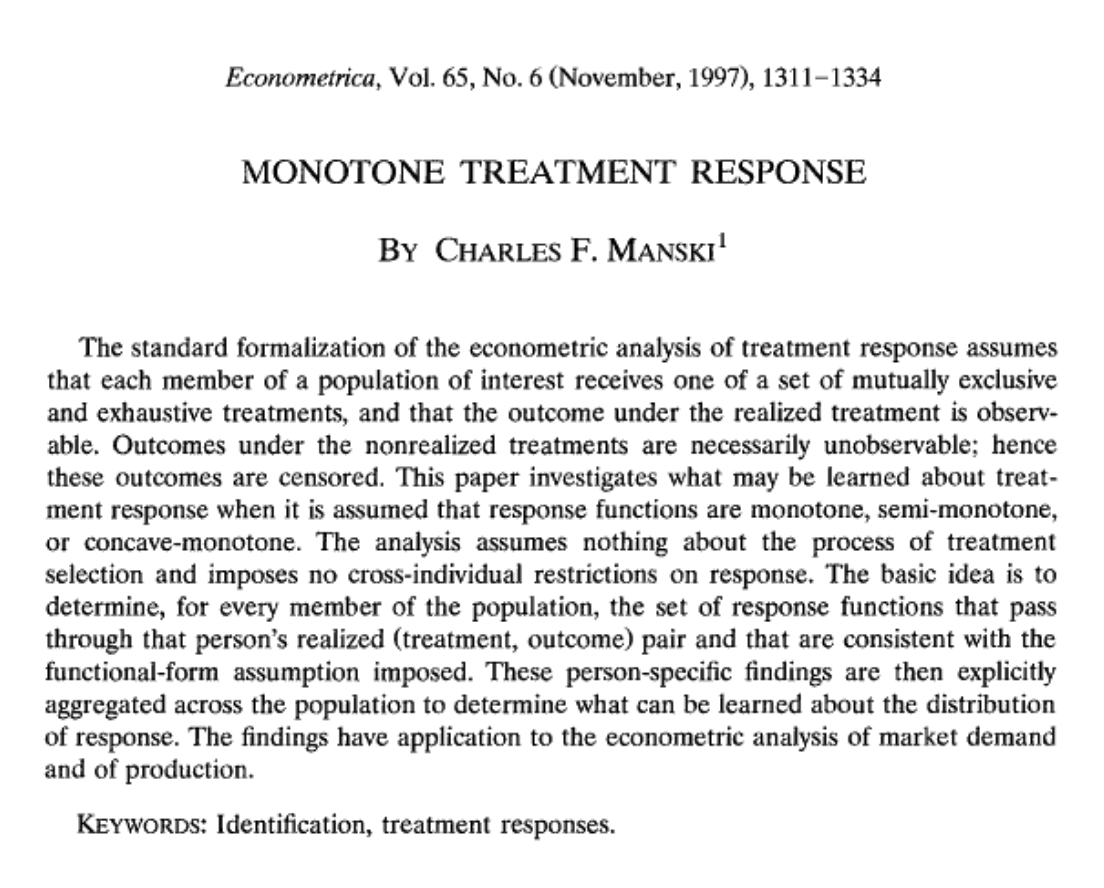
\includegraphics[width=\linewidth]{images/manski_mtr_1.png}
%       \end{column}%
%     \end{columns}
% \end{frame}


\begin{frame}{So why don't people use it more?}
      \begin{columns}[onlytextwidth, T] % align columns
        \begin{column}{.5\textwidth}
          \begin{wideitemize}
          \item These approaches seem quite powerful -- perhaps we can
            still say useful things with less assumptions
          \item Manski and Molinari (2021) recently take this approach
            thinking about identifying the share of the population
            that has been infected with Covid-19
            \begin{itemize}
            \item A huge issue that is plagued with a host of selection problems!
            \end{itemize}
          \item Make some initial assumptions on the relationship
            between testing, symptoms and positive cases, rather than
            modeling the full thing in a parametric form (e.g. SIR
            model)
          \end{wideitemize}
      \end{column}%
      \hfill%
      \begin{column}{.5\textwidth}
        
\includegraphics[width=\linewidth]{images/manski_molinari_1.png}
      \end{column}%
    \end{columns}

  \end{frame}

  
\begin{frame}{So why don't people use it more?}
      \begin{columns}[onlytextwidth, T] % align columns
        \begin{column}{.5\textwidth}
          \begin{wideitemize}
          \item Well, the problem is that the bounds are \emph{sort of} informative, but sort of not...
            \begin{itemize}
            \item $[0.001,0.525]$ is a pretty wide range of infection rates
            \end{itemize}
          \item Bit of a Rorschach test: this is either a feature or a
            bug
            \begin{itemize}
            \item Reflects how strong the parametric assumptions are
            \item Reflects how uninformed the policymaker is
            \end{itemize}
          \item It is very challenging to present bounds that are this
            uninformative in resarch papers
            \begin{itemize}
            \item Good goal is as a supplement
            \item Less true in IO style settings!
            \end{itemize}
          \end{wideitemize}
      \end{column}%
      \hfill%
      \begin{column}{.5\textwidth}
        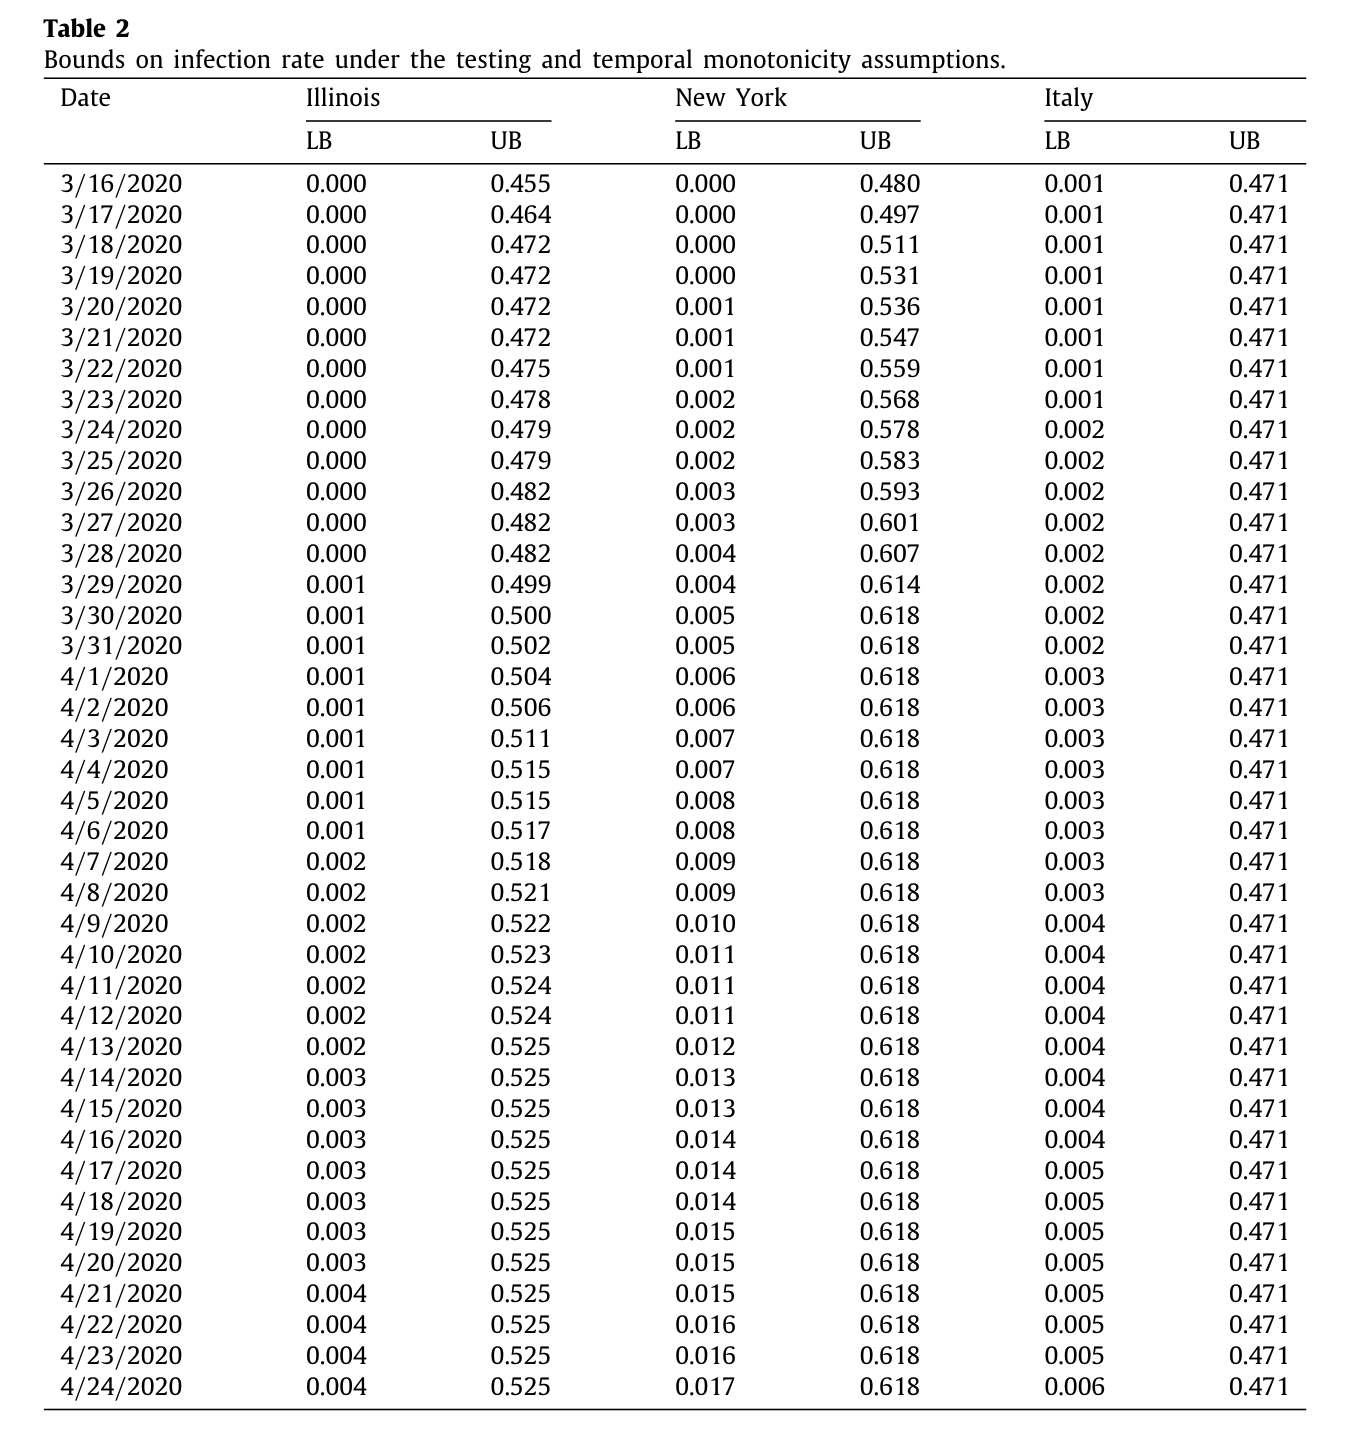
\includegraphics[width=\linewidth]{images/manksi_molinari_2.png}
      \end{column}%
    \end{columns}
\end{frame}

  
\begin{frame}{Recommended further reading}
      \begin{columns}[onlytextwidth, T] % align columns
        \begin{column}{.5\textwidth}
          \begin{wideitemize}
          \item ``Identification for Prediction and Decision'' (Manski 2007)
          \item ``Partial Identification of Local Average Treatment
            Effects With an Invalid Instrument'' Flores and
            Flores-Lagunes (2013)
          \item ``Estimation and Confidence Regions for Parameter Sets
            in Econometric Models'' Chernozhukov, Hong and Tamer
            (2007)
          \end{wideitemize}
      \end{column}%
      \hfill%
      \begin{column}{.5\textwidth}
        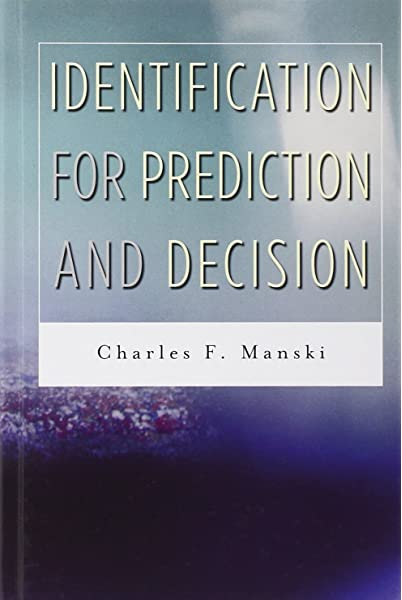
\includegraphics[width=\linewidth]{images/manski_book.jpeg}
      \end{column}%
    \end{columns}
\end{frame}


\end{document}